\section{Skalieren von Bildern}
\label{scale_Algos}
OpenFace arbeitet laut Angabe im Paper \cite{OpenFace} am besten auf Gesichtern mit einer Größe von 100 Pixel, daher werden die Bildbereiche auf diese Größe gebracht. Dies ist notwendig, ba die Berechnungen meist auf recht kleinen Bildausschnitten ausgeführt werden muss.\\
Dabei ist es wichtig, dass die Gesichtsmerkmale möglichst gut rekonstruiert werden, um die entsprechenden Landmarks zu bestimmen, dabei erhöht sich der Informationsgehalt der Bilder nicht, sie sind nur besser nutzbar, da sie dem Trainingsdatensatz stärker ähneln.\\
Die von MTCNN gelieferten und vergrößerten Boxen werden auf $130 \times 180$ Pixel gebracht, damit das beinhaltete Gesicht auf der gewünschte Größe dargestellt wird. Neben der Skalierung des Bildausschnittes muss bekannt sein, wie Punkte im skalierten Bildausschnitt in das Frame überführt werden können, damit dies bei späteren Berechnungen berücksichtigt wird.\\
Der Skalierungsfaktor ist für jeden Bildausschnitt individuell und kann sich über die Zeit ändern, wenn sich z.B. die Distanz zwischen Person und Kamera ändert. Von einer zu starken Vergrößerung ist abzuraten, da sich der Rechenaufwand pro Gesicht erhöht und die Zuverlässigkeit der Berechnungen von OpenFace sinkt, z.B. durch Falschdetektion.
\subsection{Bicubic-Skalierung}
Der neue Farbwert wird ermitteln, indem die umliegenden $4\times 4$ Pixelwerte betrachtet werden um den Farbverlauf als eine Funktion 3. Grades zu bestimmen. Somit werden feinere Details besser dargestellt als beim linearen Verfahren und Kanten bleiben eher erhalten. Allerdings kann es durch den bestimmten Verlauf auch zum Überschwingen kommen, wodurch Fehlfarben entstehen können. Ein Beispiel als Ergebnis dieses Verfahrens ist in \autoref{img_Bicubic} zu sehen.\\
\cite{wiki_Bicubic}
\subsection{Lanczos-Skalierung}
Dieser Filter basiert auf einem bewerteten Durchschnitt der umliegenden Pixel um den neuen Pixelwert zu erhalten. Die Bewertung der einzelnen Pixel wird durch eine Sinc-Funktion bestimmt, damit weiter entferntere Pixel schwächer bewertet werden als näher liegende, siehe \autoref{img_Lanczos}.\\
Die Funktion kann und wird für die Anwendung auf einen $8\times 8$ Pixel großen Bereich begrenzt. Außerdem wird durch den Kurvenverlauf der Bewertungsfunktion eine gewisse Bildschärfe erreicht.\\
\cite{wiki_Lanczos}
\[ L(x)= \left\{ \begin{array}{ll}
\frac{\sin(\pi x)}{\pi x} \cdot \frac{\sin(\pi \frac{x}{a})}{\pi \frac{x}{a}} & \textrm{wenn } -a < x <a, a\ne 0\\
1 & \textrm{wenn } x = 0\\
0 & \textrm{sonst}
\end{array}\right. \]
\subsection{Linear-Skalierung}
Um den neuen Farbwert zu ermitteln, wird zwischen den nächstgelegenen umliegenden Pixel linear Interpoliert, wodurch weitere Farbwerte entstehen. Das Ergebnis ist gleichmäßiger als Neares Neighbor, und dennoch ein recht einfaches Verfahren. Die Kanten wirken allerdings unscharf, siehe \autoref{img_Linear}.
\subsection{Nearest-Neighbor-Skalierung}
Dieses Verfahren verwendet als neuer Farbwert, den gleichen Wert wie das nächstgelegene Pixel. Dadurch werden nur die ehemaligen Pixel größer und das Gesicht wirkt sehr Kantig, da keine neuen Farbwerte bestimmt werden, siehe \autoref{img_NN}. Bei der Vergrößerung des Schachbretts sind kein Farbfehler aufgetreten, da nur zwei Farben vorhanden und Positionsabhängig sind.
\begin{figure}
	\centering
	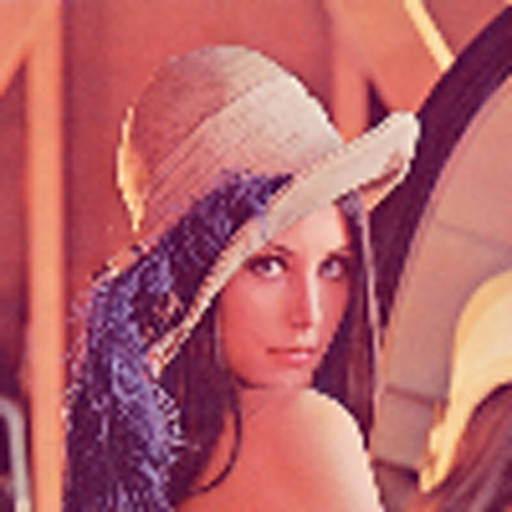
\includegraphics[width=0.2\linewidth]{img/lena100_CUBIC}
	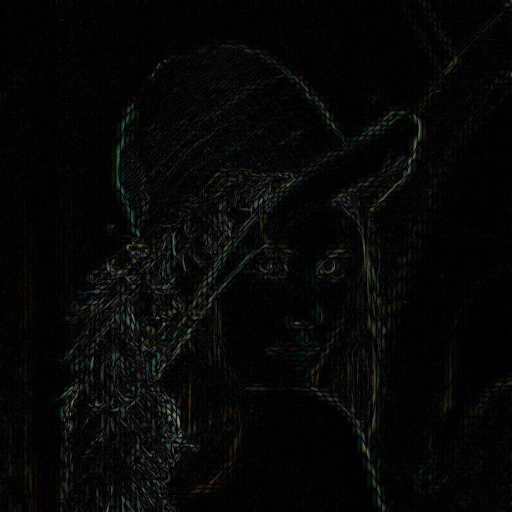
\includegraphics[width=0.2\linewidth]{img/lena100_CUBIC_differenz}
	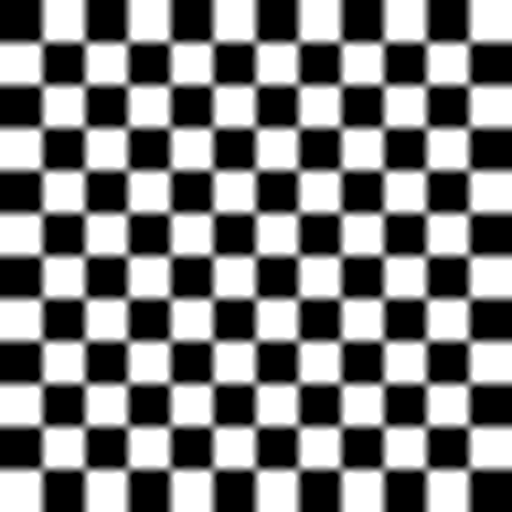
\includegraphics[width=0.2\linewidth]{img/Schachbrett_CUBIC}
	\caption{Die ursprüngliche Abbildung von Lena betrug 100 Pixel Kantenlänge und beim Schachbrett 48 Pixel, beide wurden mittels bikubischem Verfahren auf 512 Pixel vergrößert und bei Lena die Differenz zum originalen Lena-Bild bestimmt}
	\label{img_Bicubic}
\end{figure}
\begin{figure}
	\centering
	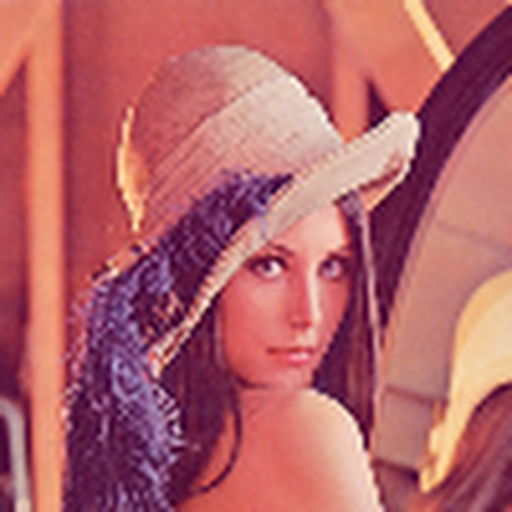
\includegraphics[width=0.2\linewidth]{img/lena100_LANCZOS4}
	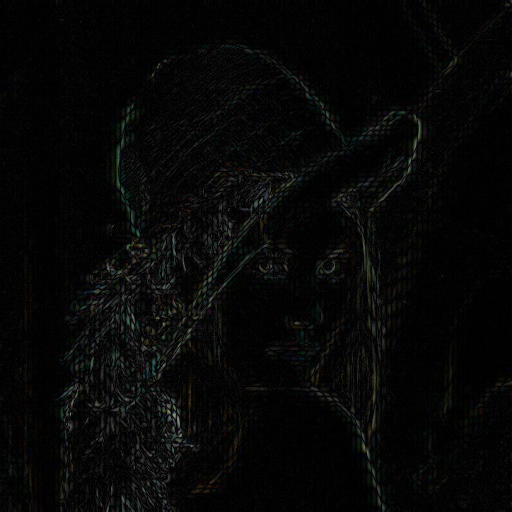
\includegraphics[width=0.2\linewidth]{img/lena100_LANCZOS4_differenz}
	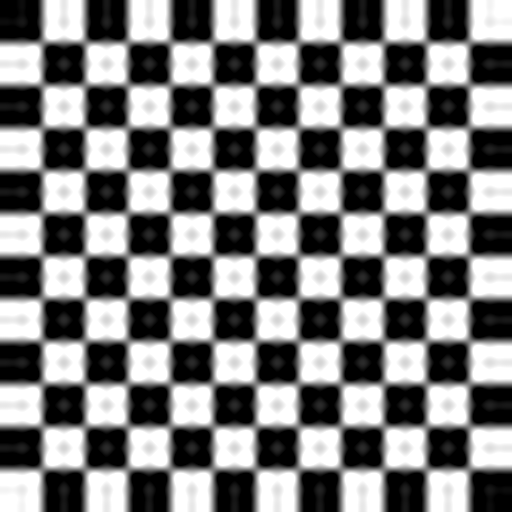
\includegraphics[width=0.2\linewidth]{img/Schachbrett_LANCZOS4}
	\caption{Die ursprüngliche Abbildung von Lena betrug 100 Pixel Kantenlänge und beim Schachbrett 48 Pixel, beide wurden mittels Lanczus-Verfahren auf 512 Pixel vergrößert und bei Lena die Differenz  zum originalen Lena-Bild bestimmt}
	\label{img_Lanczos}
\end{figure}
\begin{figure}
	\centering
	
\includegraphics[width=0.2\linewidth]{img/lena100_LINEAR}
	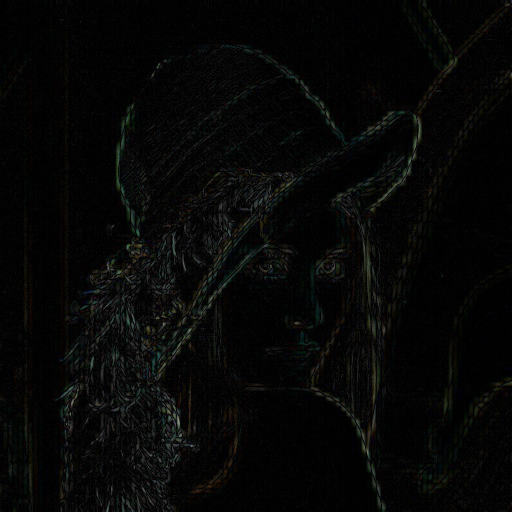
\includegraphics[width=0.2\linewidth]{img/lena100_LINEAR_differenz}
	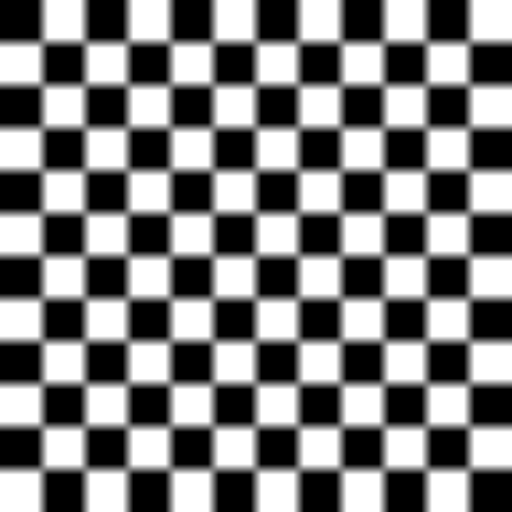
\includegraphics[width=0.2\linewidth]{img/Schachbrett_LINEAR}
	\caption{Die ursprüngliche Abbildung von Lena betrug 100 Pixel Kantenlänge und beim Schachbrett 48 Pixel, beide wurden mittels linearer Interpolation auf 512 Pixel vergrößert und bei Lena die Differenz zum originalen Lena-Bild bestimmt}
	\label{img_Linear}
\end{figure}
\begin{figure}
	\centering
	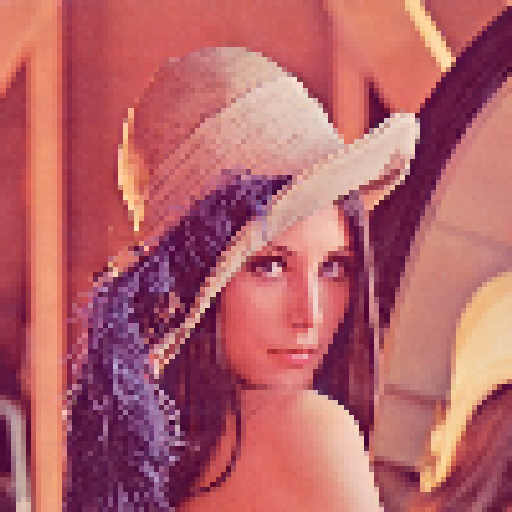
\includegraphics[width=0.2\linewidth]{img/lena100_NN}
	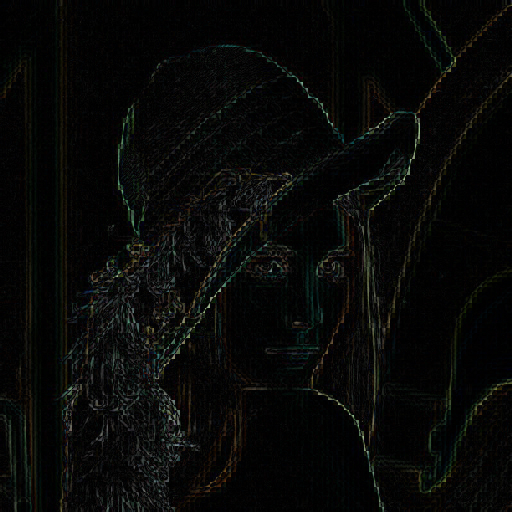
\includegraphics[width=0.2\linewidth]{img/lena100_NN_differenz}
	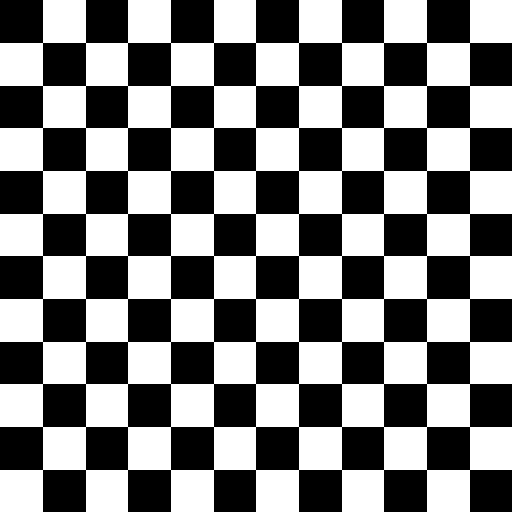
\includegraphics[width=0.2\linewidth]{img/Schachbrett_NN}
	\caption{Die ursprüngliche Abbildung von Lena betrug 100 Pixel Kantenlänge und beim Schachbrett 48 Pixel, beide wurden mittels Nearest-Neighbor auf 512 Pixel vergrößert und bei Lena die Differenz zum originalen Lena-Bild bestimmt}
	\label{img_NN}
\end{figure}
% http://docs.opencv.org/2.4/modules/imgproc/doc/geometric_transformations.html#resize
\subsection{Qualität der Skalierung}
Nun wird die Auswirkung der verschieden Skalierungsverfahren auf die Qualität der Berechnung untersucht. Dazu wurde der <Datensatz> verwendet, linear um den angegebenen Faktor verkleinert und mittels der angegebenen Verfahren wieder vergrößert und von OpenFace ausgewertet.
\subsubsection{Position}
Als erstes werden die berechnete Distanzen mit denen des Datensatzes verglichen. In \autoref{img_X_Pos_Skal} ist die Abweichung entlang der X-Achse dargestellt. Nearest-Neighbor liefert die genauesten Ergebnisse, auch wenn die Detektion früher ausfällt als die der anderen drei.\\
Auf der Y-Achse ist das Lineare-Verfahren etwas besser als die der Anderen, das Nearest-Neighbor ist hierbei überraschend das Schlechteste, siehe \autoref{img_Y_Pos_Skal}.\\
Nur schwer zu erkennen da der Unterschied minimal ausfällt, ist bei der Bestimmung der Z-Position das Nearest-Neighbor-Verfahren ebenfalls am Besten, siehe \autoref{img_Z_Pos_Skal}. Die anderen drei liefern nahezu eine identisch Qualität. Bei sehr kleinen Skalierungen existieren durchaus auch sehr große Fehler, diese wurden allerdings bei der Darstellung abgeschnitten, da bei dieser Größe die Detektionsrate so klein ist, dass sie nahezu irrelevant werden.
\begin{figure}
	\centering
	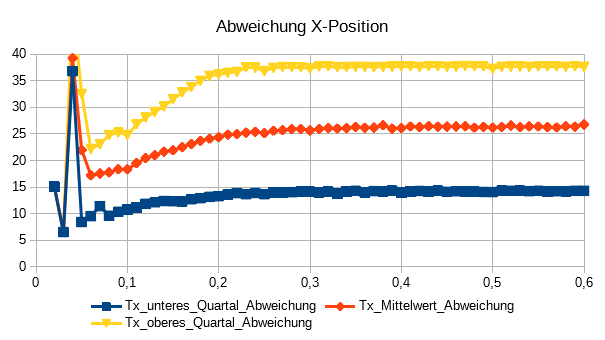
\includegraphics[width=0.45\linewidth]{tabelle2/X_Pos_Cubic}
	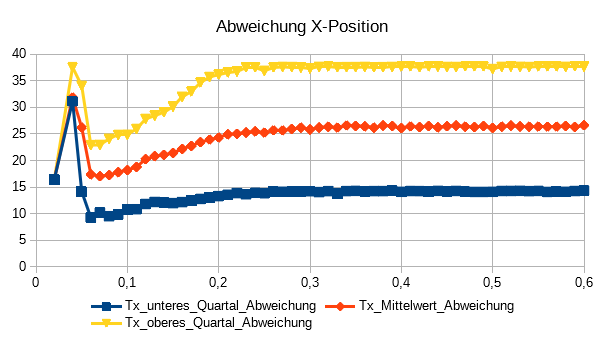
\includegraphics[width=0.45\linewidth]{tabelle2/X_Pos_Lanc}
	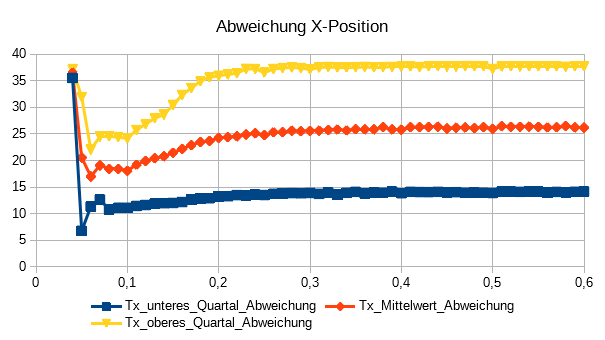
\includegraphics[width=0.45\linewidth]{tabelle2/X_Pos_Linear}
	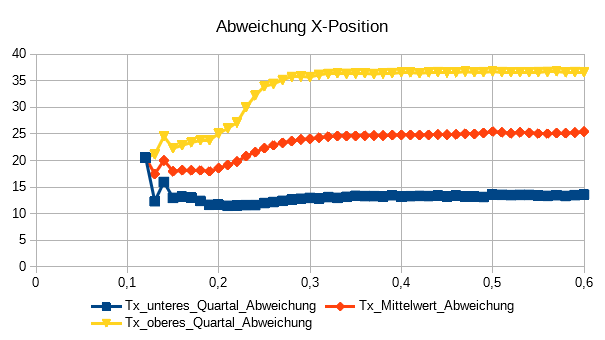
\includegraphics[width=0.45\linewidth]{tabelle2/X_Pos_NN}
	\caption{Zusammenhang zwischen der Skalierung (X-Achse) und der Abweichung in X-Richtung (Y-Achse) in Millimeter. 
		Bicubic (oben links), Lanczos (oben rechts), Linear (unten links), Nearest-Neighbor (unten rechts)}
	\label{img_X_Pos_Skal}
\end{figure}
\begin{figure}
	\centering
	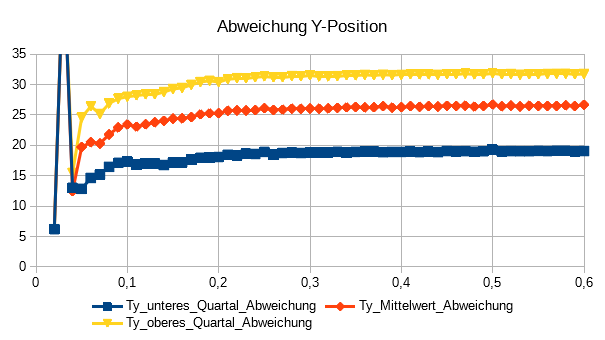
\includegraphics[width=0.45\linewidth]{tabelle2/Y_Pos_Cubic}
	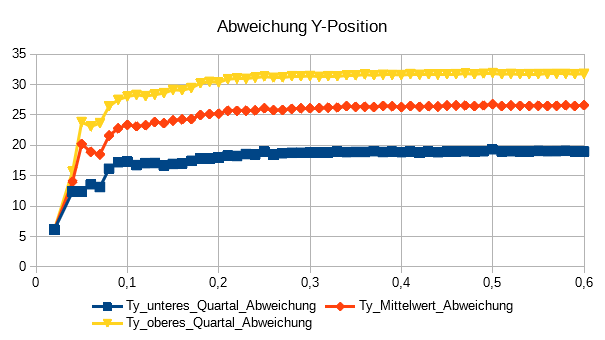
\includegraphics[width=0.45\linewidth]{tabelle2/Y_Pos_Lanc}
	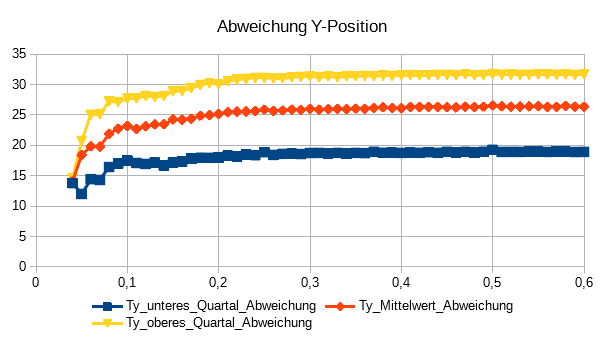
\includegraphics[width=0.45\linewidth]{tabelle2/Y_Pos_Linear}
	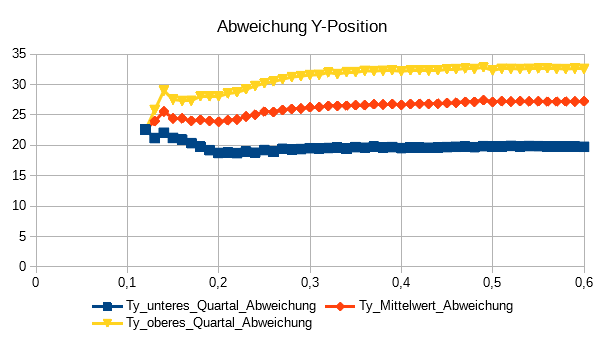
\includegraphics[width=0.45\linewidth]{tabelle2/Y_Pos_NN}
	\caption{Zusammenhang zwischen der Skalierung (X-Achse) und der Abweichung in Y-Richtung (Y-Achse) in Millimeter. 
		Bicubic (oben links), Lanczos (oben rechts), Linear (unten links), Nearest-Neighbor (unten rechts)}
	\label{img_Y_Pos_Skal}
\end{figure}
\begin{figure}
	\centering
	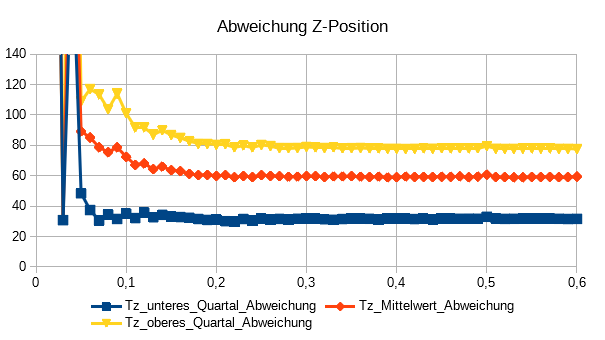
\includegraphics[width=0.45\linewidth]{tabelle2/Z_Pos_Cubic}
	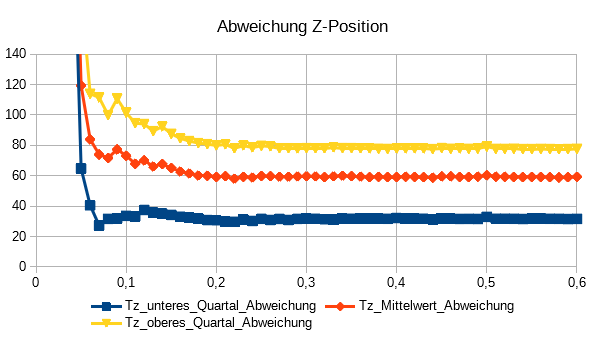
\includegraphics[width=0.45\linewidth]{tabelle2/Z_Pos_Lanc}
	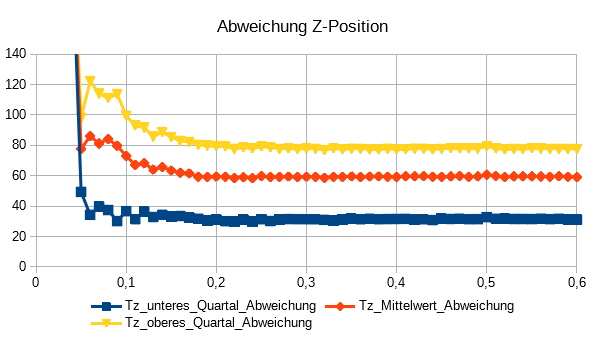
\includegraphics[width=0.45\linewidth]{tabelle2/Z_Pos_Linear}
	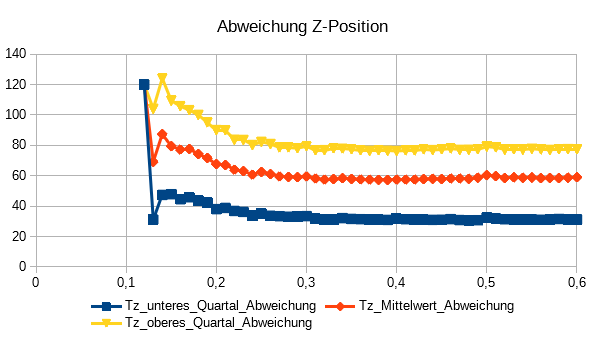
\includegraphics[width=0.45\linewidth]{tabelle2/Z_Pos_NN}
	\caption{Zusammenhang zwischen der Skalierung (X-Achse) und der Abweichung in Z-Richtung (Y-Achse) in Millimeter. 
		Bicubic (oben links), Lanczos (oben rechts), Linear (unten links), Nearest-Neighbor (unten rechts)}
	\label{img_Z_Pos_Skal}
\end{figure}
\subsubsection{Orientierung}
Des weiteren wird der berechneten Winkel um die jeweilige Achse betrachtet und mit den korrekten verglichen. Die geringste Abweichung bei der bestimung der X-Rotation liefert Nearest-Neighbor, siehe \autoref{img_X_Rot_Skal}. Auffällig ist außerdem der kleinere Wertebereich des Linearen-Verfahrens.\\
Auch bei der Y-Rotation schneidet Nearest-Neighbor am besten ab, siehe \autoref{img_Y_Rot_Skal}, allerdings sind die unterscheide minimal.\\
Bei der Z-Rotation ist kein erkennbarer Unterschied zwischen den einzelnen Verfahren, wobei bei Nearest-Neighbor deutlich früher der Wertebereich sinkt.
\begin{figure}
	\centering
	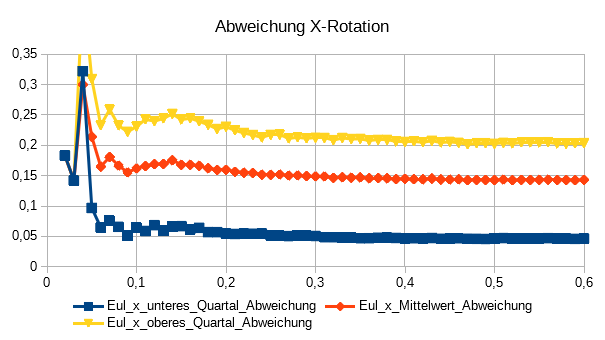
\includegraphics[width=0.45\linewidth]{tabelle2/X_Rot_Cubic}
	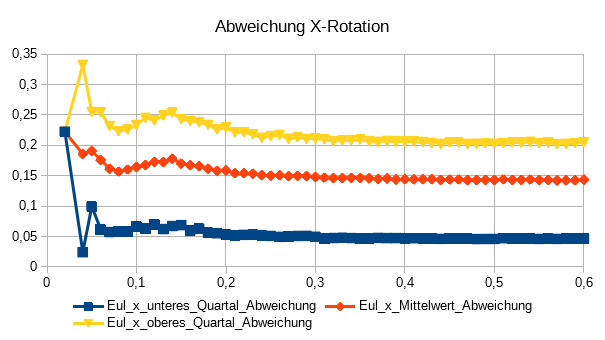
\includegraphics[width=0.45\linewidth]{tabelle2/X_Rot_Lanc}
	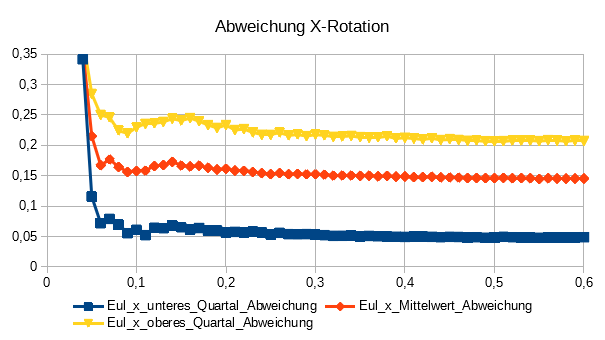
\includegraphics[width=0.45\linewidth]{tabelle2/X_Rot_Linear}
	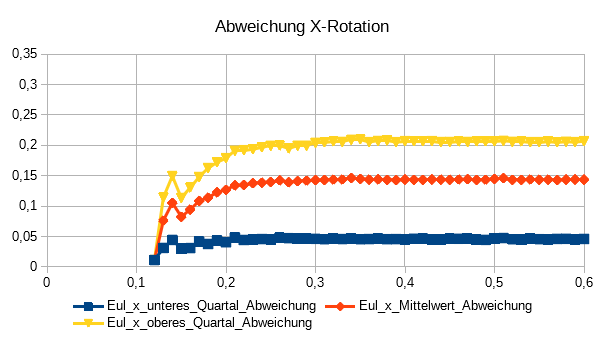
\includegraphics[width=0.45\linewidth]{tabelle2/X_Rot_NN}
	\caption{Zusammenhang zwischen der Skalierung (X-Achse) und der Abweichung des Winkels in X-Richtung, Angabe in Bogenmaß. 
		Bicubic (oben links), Lanczos (oben rechts), Linear (unten links), Nearest-Neighbor (unten rechts)}
	\label{img_X_Rot_Skal}
\end{figure}
\begin{figure}
	\centering
	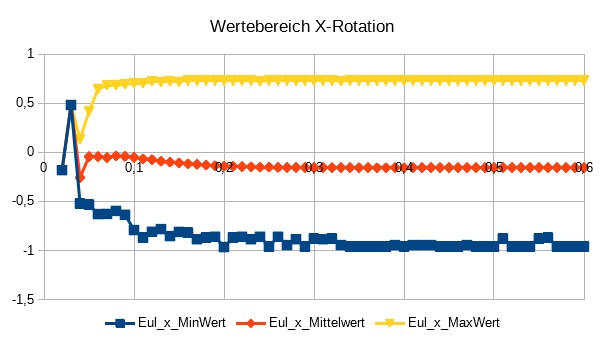
\includegraphics[width=0.45\linewidth]{tabelle2/X_Rot_Val_Cubic}
	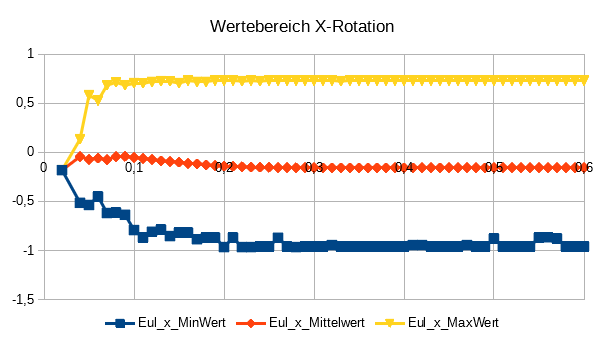
\includegraphics[width=0.45\linewidth]{tabelle2/X_Rot_Val_Lanc}
	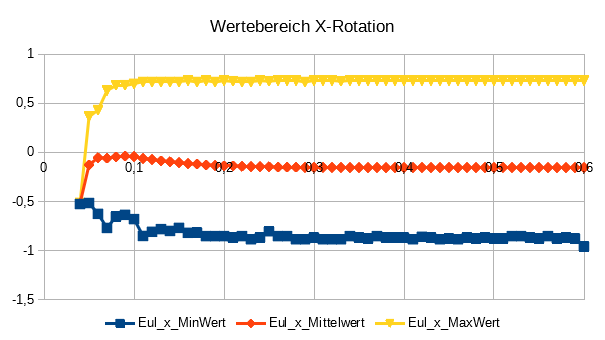
\includegraphics[width=0.45\linewidth]{tabelle2/X_Rot_Val_Linear}
	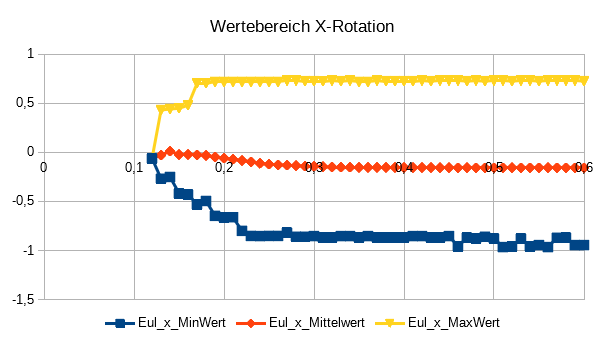
\includegraphics[width=0.45\linewidth]{tabelle2/X_Rot_Val_NN}
	\caption{Zusammenhang zwischen der Skalierung (X-Achse) und der Abweichung des Winkels in X-Richtung, Angabe in Bogenmaß. 
		Bicubic (oben links), Lanczos (oben rechts), Linear (unten links), Nearest-Neighbor (unten rechts)}
	\label{img_X_Rot_Val_Skal}
\end{figure}
\begin{figure}
	\centering
	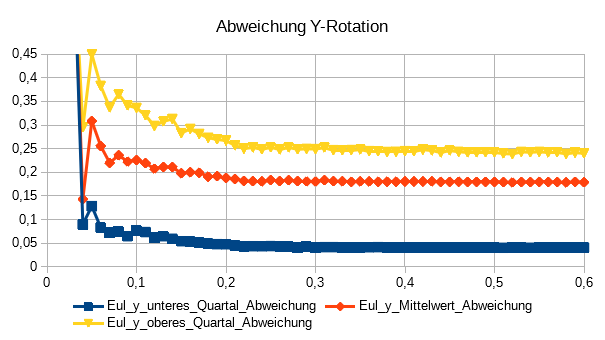
\includegraphics[width=0.45\linewidth]{tabelle2/Y_Rot_Cubic}
	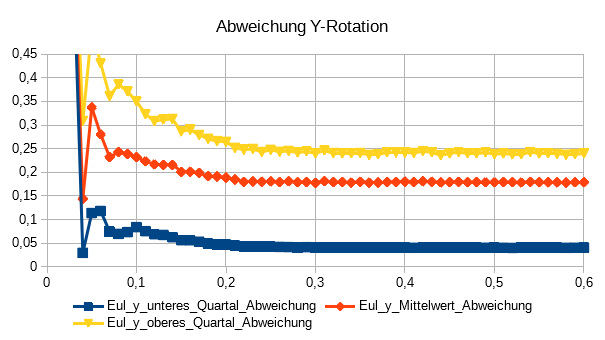
\includegraphics[width=0.45\linewidth]{tabelle2/Y_Rot_Lanc}
	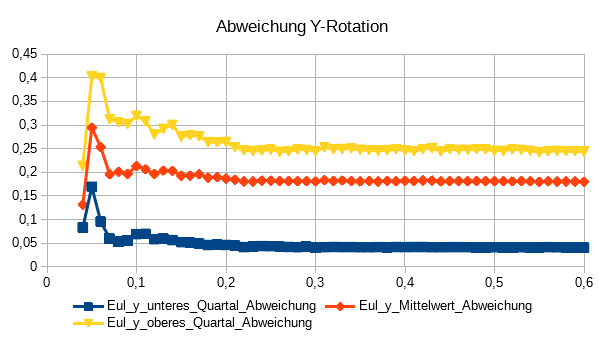
\includegraphics[width=0.45\linewidth]{tabelle2/Y_Rot_Linear}
	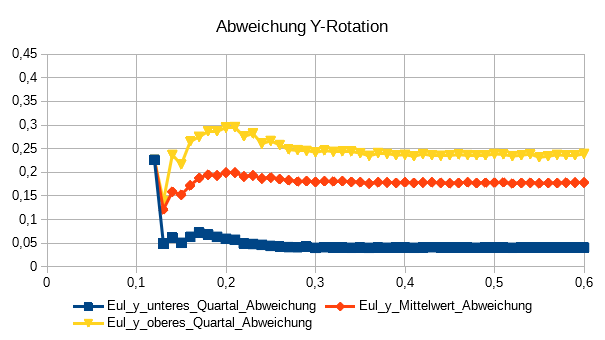
\includegraphics[width=0.45\linewidth]{tabelle2/Y_Rot_NN}
	\caption{Zusammenhang zwischen der Skalierung (X-Achse) und der Abweichung des Winkels in Y-Richtung, Angabe in Bogenmaß.
		Bicubic (oben links), Lanczos (oben rechts), Linear (unten links), Nearest-Neighbor (unten rechts)}
	\label{img_Y_Rot_Skal}
\end{figure}
\begin{figure}
	\centering
	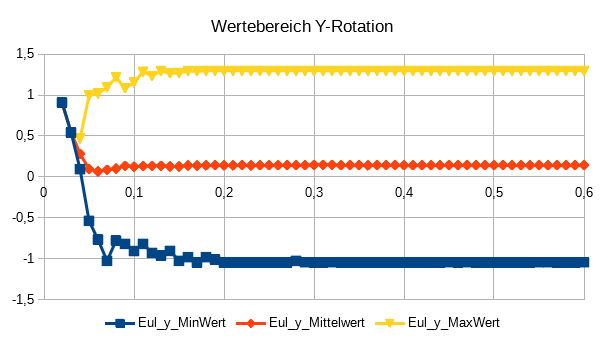
\includegraphics[width=0.45\linewidth]{tabelle2/Y_Rot_Val_Cubic}
	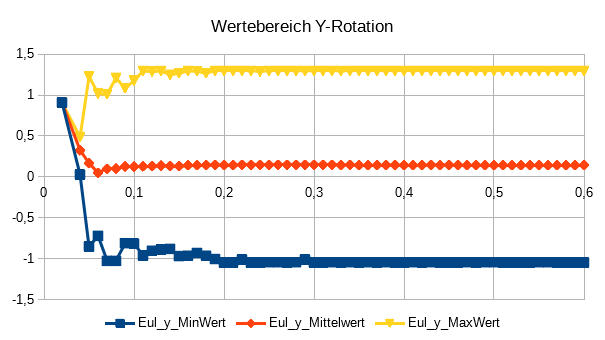
\includegraphics[width=0.45\linewidth]{tabelle2/Y_Rot_Val_Lanc}
	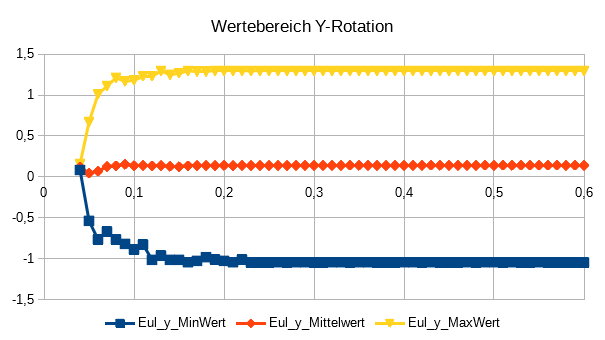
\includegraphics[width=0.45\linewidth]{tabelle2/Y_Rot_Val_Linear}
	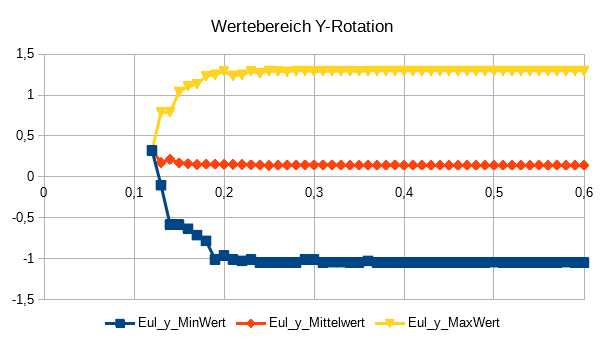
\includegraphics[width=0.45\linewidth]{tabelle2/Y_Rot_Val_NN}
	\caption{Zusammenhang zwischen der Skalierung (X-Achse) und der Wertebereich des Winkels in Y-Richtung, Angabe in Bogenmaß.
		Bicubic (oben links), Lanczos (oben rechts), Linear (unten links), Nearest-Neighbor (unten rechts)}
	\label{img_Y_Rot_Val_Skal}
\end{figure}
\begin{figure}
	\centering
	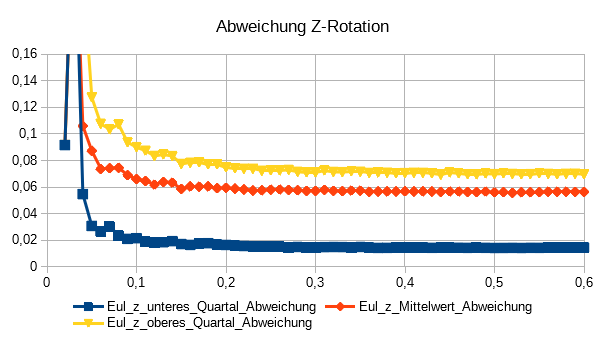
\includegraphics[width=0.45\linewidth]{tabelle2/Z_Rot_Cubic}
	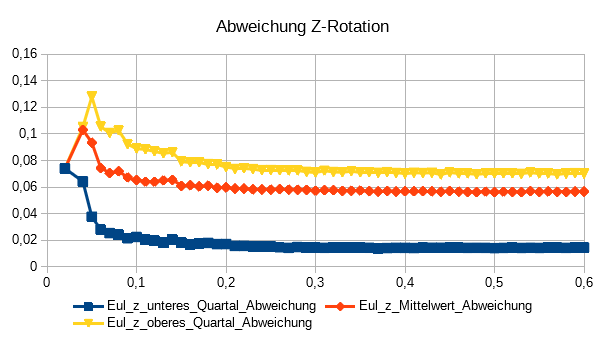
\includegraphics[width=0.45\linewidth]{tabelle2/Z_Rot_Lanc}
	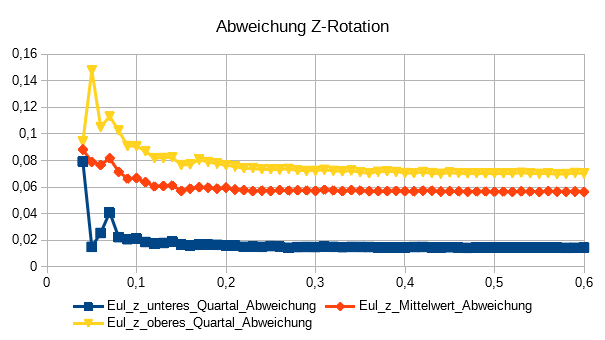
\includegraphics[width=0.45\linewidth]{tabelle2/Z_Rot_Linear}
	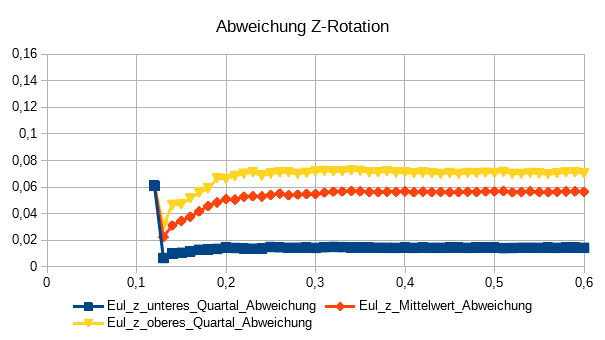
\includegraphics[width=0.45\linewidth]{tabelle2/Z_Rot_NN}
	\caption{Zusammenhang zwischen der Skalierung (X-Achse) und der Abweichung des Winkels in Z-Richtung, Angabe in Bogenmaß.
		Bicubic (oben links), Lanczos (oben rechts), Linear (unten links), Nearest-Neighbor (unten rechts)}
	\label{img_Z_Rot_Skal}
\end{figure}
\begin{figure}
	\centering
	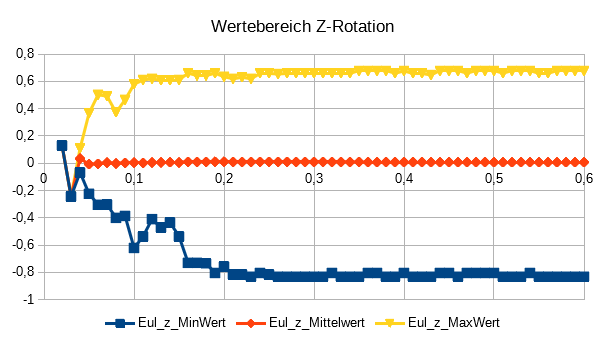
\includegraphics[width=0.45\linewidth]{tabelle2/Z_Rot_Val_Cubic}
	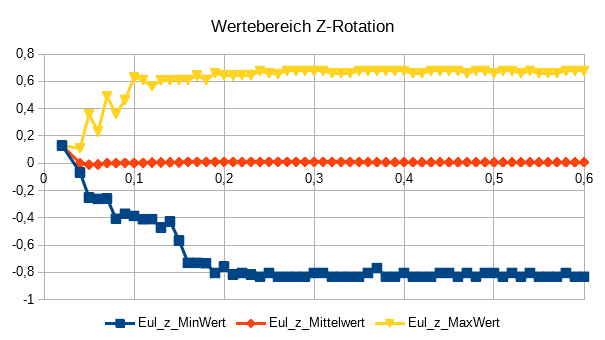
\includegraphics[width=0.45\linewidth]{tabelle2/Z_Rot_Val_Lanc}
	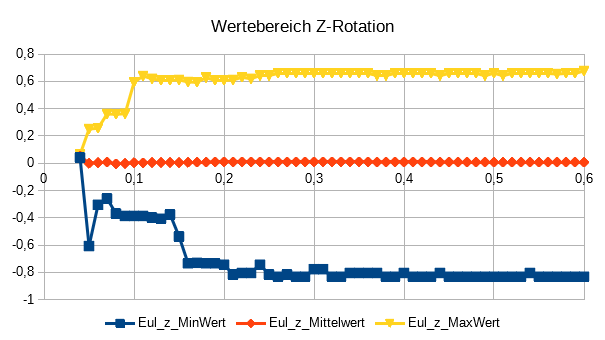
\includegraphics[width=0.45\linewidth]{tabelle2/Z_Rot_Val_Linear}
	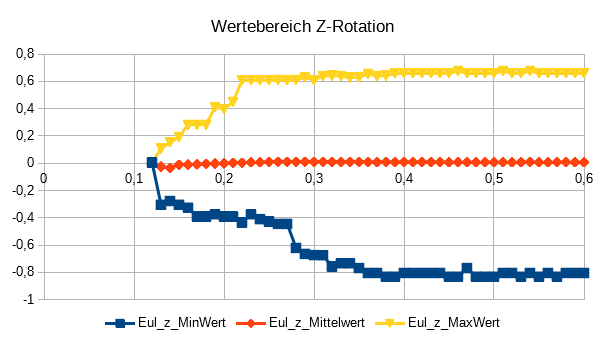
\includegraphics[width=0.45\linewidth]{tabelle2/Z_Rot_Val_NN}
	\caption{Zusammenhang zwischen der Skalierung (X-Achse) und der Wertebereiche des Winkels in Z-Richtung, Angabe in Bogenmaß.
		Bicubic (oben links), Lanczos (oben rechts), Linear (unten links), Nearest-Neighbor (unten rechts)}
	\label{img_Z_Rot_Val_Skal}
\end{figure}
\subsection{Ergebnisse Angeben}
Es zeigt sich, dass bei der Analyse von Gesichter das Nearest-Neighbor Verfahren die genauesten Ergebnisse liefert. Allerdings ist der Arbeitsbereich deutlich eingeschränkter als im Vergleich zu den anderen Verfahren. Die benötigte Mindestgröße des Gesichts im Orginal und dem geringen Wertebereich im Bezug auf die Rotationen zeigt, das dieses Verfahren eher ungeeignet ist.\\
Bei dem Linearen-Verfahren ist die Abweichung bei den Rotationen am größten, auch wenn es sich nur um etwa ein halbes Grad handelt. Zwischen dem Bicubic- und Lanczos-Verfahren gibt es in den relevanten Bereichen keinen signifikanten Unterschied, wobei das Lanczos in den kleineren Bereichen gleichmäßigere Ergebnisse. Somit kann die Wahl des Verfahrens vom Rechenaufwand abhängig gemacht werden.\\
ToDo: Bessere Auswertung\\
Bicubig am besten